% !TEX encoding = UTF-8 Unicode
% !TEX root = SystemTemplate.tex

\documentclass{book}
% !TEX root = SystemTemplate.tex

\usepackage[width=6.5in, height=9.2in, top=1.0in, papersize={8.5in,11in}]{geometry}
\usepackage[pdftex]{graphicx}
%\usepackage{draftwatermark}
\usepackage{amsmath}
\usepackage{amsthm}
\usepackage{amssymb}
%\usepackage{txfonts}
\usepackage{textcomp}
%\usepackage{amsthm}

\usepackage[all]{xy}
\usepackage{fancyhdr}
\pagestyle{fancy}
\usepackage{hyperref}
\usepackage{verbatim}
\usepackage{algorithm}
\usepackage{algorithmic}
\usepackage{array}
\usepackage{color}
\usepackage{listings}
\lstset{language=c,frame=ltrb,framesep=5pt,basicstyle=\normalsize,
 keywordstyle=\ttfamily\color{DarkRed},
identifierstyle=\ttfamily\color{DarkBlue}\bfseries,
commentstyle=\color{OliveGreen},
stringstyle=\ttfamily,
showstringspaces=false,tabsize = 3}
\usepackage{calc}
\usepackage{doxygen}
\usepackage[utf8]{inputenc}
\usepackage{makeidx}
\usepackage{multicol}
\usepackage{multirow}
\usepackage[table]{xcolor}

\definecolor{color02}{rgb}{0.18,0.35,0.59}
\definecolor{color03}{rgb}{0.44,0.59,0.82}
\definecolor{color06}{rgb}{0.35,0.35,0.35}


\newtheorem{summary}{Summary:}
\newtheorem{example}{Example:}


\definecolor{OliveGreen}{cmyk}{0.64,0,0.95,0.40}
\definecolor{DarkBlue}{cmyk}{0.76,0.76,0,0.20}
\definecolor{DarkRed}{cmyk}{0,1,1,0.45}


\def      \RR             {{\mathbb R}} 
\def      \DS            {\displaystyle} 

\setlength{\oddsidemargin}{0mm} 
\setlength{\evensidemargin}{0mm} 

%\SetWatermarkLightness{0.975}
%\SetWatermarkScale{6}
%\SetWatermarkText{\includegraphics{test.png}}

\pagestyle{fancy}
\renewcommand{\chaptermark}[1]{\markboth{#1}{}}
\renewcommand{\sectionmark}[1]{\markright{\thesection\ #1}}
\fancyhf{}
\fancyhead[LE,RO]{\bfseries\thepage}
\fancyhead[LO]{\bfseries\rightmark}
\fancyhead[RE]{\bfseries\leftmark}
\fancyfoot[LE,RO]{Confidential and Proprietary}
%\renewcommand{\headrulewidth}{0.5pt}
%\renewcommand{\footrulewidth}{0pt}
%\addtolength{\headheight}{0.5pt}
%\setlength{\footskip}{0mm}
%\renewcommand{\footruleskip}{0pt}


\definecolor{MSBlue}{rgb}{.204,.353,.541}
\definecolor{MSLightBlue}{rgb}{.31,.506,.741}
\definecolor{MSBlue1}{rgb}{0.18,0.35,0.59}
\definecolor{MSBlue2}{rgb}{0.44,0.59,0.82}
\definecolor{MSBlue3}{rgb}{0.35,0.35,0.35}


\usepackage{titlesec}
\titleformat{\chapter}[display]
{\normalfont\bfseries\color{MSBlue1}}    %\normalfont\bfseries\filcenter}
{\LARGE\thechapter}
{1ex}
{\titlerule[2pt]
\vspace{2ex}%
\LARGE}
[\vspace{1ex}%
{\titlerule[2pt]}]

\definecolor{MSBlue}{rgb}{.204,.353,.541}
\definecolor{MSLightBlue}{rgb}{.31,.506,.741}
\definecolor{MSBlue1}{rgb}{0.18,0.35,0.59}
\definecolor{MSBlue2}{rgb}{0.44,0.59,0.82}
\definecolor{MSBlue3}{rgb}{0.35,0.35,0.35}

%\titleformat*{\section}{\Large\bfseries\sffamily\color{MSBlue}}
%\titleformat*{\subsection}{\large\bfseries\sffamily\color{MSLightBlue}}
%\titleformat*{\section}{\Large\bfseries\color{MSBlue1}}
%\titleformat*{\subsection}{\large\bfseries\color{MSBlue2}}

\titleformat*{\section}{\Large\bfseries\color{MSBlue}}
\titleformat*{\subsection}{\large\bfseries\color{MSLightBlue}}
\titleformat*{\subsubsection}{\large\bfseries\color{MSBlue3}}
\setcounter{secnumdepth}{3}
\renewcommand{\thesubsubsection}{\thesubsection.\alph{subsubsection}}

 % This sets the format.

% Add your title page contents here 
\title{{\color{MSBlue1} \rule{\linewidth}{0.5mm}}\\[2mm] {\huge \bfseries \color{MSBlue1} Program Tester Sprint 2 }\\[-1mm] {\color{MSBlue1}\rule{\linewidth}{0.5mm}} \\  \vfill
{\LARGE \bfseries \color{MSBlue2} Software Engineering Spring 2014  Documentation }\\  \vfill 
{\color{MSBlue1} Software Engineering Adventure Line} }
\author{\color{MSBlue1}  Erik Hattervig \and \color{MSBlue1} Andrew Koc \and  \color{MSBlue1} Jonathan Tomes }
\date{\color{MSBlue1} \today}


\begin{document}
\frontmatter
\maketitle


\tableofcontents
\listoffigures
\listoftables
\listofalgorithms


% !TEX root = SystemTemplate.tex

\chapter{Mission}

To create a program capable of automatically grading programs written for lower-level programming courses such as CSC150 and CSC250. Given the name of a source code file, it will compile the code and find all test cases (notated by a ".tst" extension) in the parent and any child directories of where this program's executable is located. The target program will be run against each test case and be recorded as a pass or fail based on the difference between expected and actual output. After all the tests are executed, the results, including statistics, will be written to a log file.  % add mission statement to mission.tex
% !TEX root = SystemTemplate.tex

\chapter{Document Preparation and Updates}

Current Version [3.0.0]
\vspace*{5mm}

{\color{MSBlue3}
\noindent
\textit{Prepared By:}\\
\textit{Sam Carroll}\\
\textit{Colter Assman}\\
\textit{Shaun Gruenig}\\
\textit{Erik Hattervig}\\
\textit{Andrew Koc}\\
\textit{Jonathan Tomes}\\
\textit{Joe Manke}\\
\textit{Adam Meaney}\\
}

\vfill
\noindent
{\color{color02} \textit{\textbf{Revision History}}}\\
\begin{tabular}{|>{\raggedright}p{1.5cm}|>{\raggedright}p{3cm}|>{\raggedright}p{1.5cm}|>{\raggedright}p{9cm}|}
\hline
\textit{\textbf{Date}} &  \textit{\textbf{Author}} & \textit{\textbf{Version}} & \textit{\textbf{Comments}}\tabularnewline
\hline
 \textit{\textbf{2/19/14}} & \textit{Samuel Carroll} & \textit{1.0.0} & \textit{Initial version}\tabularnewline
\hline
 \textit{\textbf{3/23/14}} & \textit{Jonathan Tomesl} & \textit{2.0.0} & \textit{Sprint 2 Version}\tabularnewline
 \hline
 \textit{\textbf{4/27/14}} & \textit{Joe Manke} & \textit{3.0.0} & \textit{Sprint 3 Version}\tabularnewline
\hline
\end{tabular}
\vfill



 
\mainmatter

%%  Add to the following chapters

% !TEX root = SystemTemplate.tex

\chapter{Overview and concept of operations}

The overview should take the form of an executive summary. Give the reader a feel for the purpose of the document, what is contained in the document, and an idea of the purpose for the system or product.


\section{Scope}
This document covers the design and implementation of the program.

\section{Purpose}
The purpose of this program is to assign pass/fail grades to simple programs run against a number of test cases. 

\subsection{Compilation}
In order to test a program, it must be compiled into an executable.

\subsection{Directory Crawl}
This component finds all of the test cases. 

\subsection{Test Execution}
The target program will be executed against a number of test cases.

\subsection{Result Logging}
Results of the tests must be recorded for the user to read.

\section{Systems Goals}
The goal of this system is to perform automated testing and grading for C++ programs.

\section{System Overview and Diagram}
The program begins by finding all test files. Then, the target program is compiled. Next, all of the test cases are executed. Finally, the results are written to the log file.

\begin{figure}[tbh]
\begin{center}
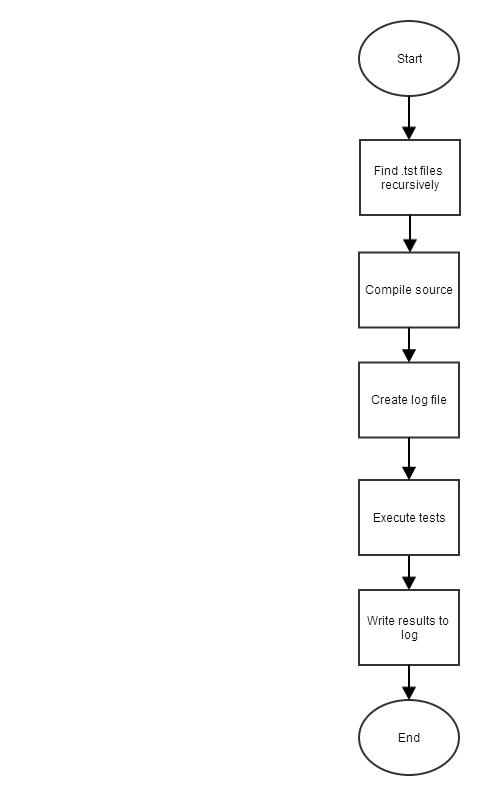
\includegraphics[width=0.75\textwidth]{./soft_eng_prog1}
\end{center}
\caption{Program flowchart \label{systemdiagram}}
\end{figure}

\section{Technologies Overview}
Developed in Linux in C++, using the g++ compiler.\newline
Documentation created using TexWorks and MikTex.\newline
Flowchart created using Gliffy.\newline

\section{Terminology and Acronyms}

See Table 1.1
\begin{table}[tbh]
\begin{center}
\begin{tabular}{|r|l|}
\hline
    GPL & General public licenced software such as GNU\textbackslash Linux environments and tools \\ \hline
    Agile Methodology & An approach to project management as it relates to software engineering \url{agilemanifesto.org} \\ \hline
    C++  STL & Standard Template Libraries: classes and methods used in common C++. \\
    \hline
\end{tabular}
\caption{Defining Some Important Terms \label{terms}}
\end{center}
\end{table}
% !TEX root = SystemTemplate.tex


\chapter{Project Overview}


\section{Team Members and Roles}
The team members of the Whitespace Cowboys were Kelsey Bellew, Ryan Brown, and Ryan Feather. 

\begin{itemize}
\item Kelsey Bellew was the Scrum Master.
\item Ryan Brown was the Product Owner.
\item Ryan Feather was the Technical Lead.
\end{itemize}

The team members of Lounge Against The Machine were Adam Meaney, Joseph Manke, and Alex Wulff.

\begin{itemize}
\item Adam Meaney was the Scrum Master.
\item Joseph Manke was the Product Owner.
\item Alex Wulff was the Technical Lead and Co-Scrum Master and Co-Product Owner.
\end{itemize}


\section{Project  Management Approach}
This project uses the Agile methodology. The sprints are three weeks in length, and the product backlog is hosted on Trello. Bug or trouble tickets are also to be posted on Trello, along with initial user stories. 


\section{Phase  Overview}
The initial phase that this project went through took us from conception to version 1.0.0 at which point the project changed to Lounge Against The Machine.  The current version, V2.0.0 has extended features such as a test generator and multiple test program support. It started with several planning talks and research into the technical challenges this project presented. Once decisions were made about the technical design of the system, development began.

In addition to technical challenges it took some time to clarify requirements and turn the provided user stories into the design of the current product.

Once the working version was established and most of the development in this sprint was done, the system and code were tested. A code review was done and several fixes were implemented accordingly, bringing us to a stable release of 1.0.0.  Version 2.0.0 was widely devised as a joke by Alex Wulff, but has since been modified into a respectable extension of the original.  Extensive testing on the test case generator has been completed in the attempt to provide the most detailed and customizable generator a customer could desire.


\section{Terminology and Acronyms}
See Table \ref{terms}
\begin{table}[tbh]
\begin{center}
\begin{tabular}{|r|l|}
\hline
    GNU and GNU Tools & The tools provided in most GNU\textbackslash Linux environments \\ \hline
    Agile Methodology & An approach to project management and software development \url{agilemanifesto.org} \\ \hline
    C++ Template Libraries & A built-in set of classes used for storing data. \\
    \hline
\end{tabular}
\caption{Defining Some Important Terms \label{terms}}
\end{center}
\end{table}

% !TEX root = SystemTemplate.tex
\chapter{User Stories, Backlog and Requirements}
\section{Overview}

This section will look at the userstories of the development of the program, the requirements
of the program, the proof of concept results, and research task results. It will also look at the
reason for developing this software. 

\subsection{Scope}

This document will contain stakeholder information, 
initial user stories, requirements, proof of concept results, and various research 
task results. 

\subsection{Purpose of the System}
To test a set of basic computer programs written in the C++ language so a grade can quickly be assigned to a class of students.
The system will also be able to generate random test cases from user input.

\section{ Stakeholder Information}

The people most interested in this project is Dr. Logar and perhaps other computer science faculty, who are looking to quickly
and easily, grade programs that are turned in by CSC 150 students.

\subsection{Customer or End User (Product Owner)}
The product owner on the first sprint was Samuel Carroll, he created a list with his teammates 
and on a day, selected by Dr. Logar, met with her and the other teams' product owner to determine
exatly what Dr. Logar wanted. Samuel was also the team member most involved in keeping the Trello 
board up to date.

The product owner on the second sprint was Erik Hattervig, he gathered the necessary requirments of the
second sprint from Dr Logar, relaied the information to his teammates, and set up the product backlog on
the Trello board.

The product owner on the third sprint was Joe Manke. He gathered requirements from Dr. Logar, created the cards on Trello, and set up the GitHub repository for the sprint.

\subsection{Management or Instructor (Scrum Master)}
The scrum master for the first sprint was Colter Assman, his duties were to ensure that the project 
stayed on track and if any team member ran into some issues he would help them get back on track.   
Colter also was responsible for the running of the daily scrum.

The scrum master for the second sprint was Jonathon Tomes,  he was in charge of managing the scheduling
for the team members, creating spring schedules, and moving tasks from the product backlog to the sprint backlog.
He also lead the scrum meetings.

The scrum master for the thrid sprint was Adam Meaney. He assigned tasks and managed the Trello board.

\subsection{Investors}
Our sole investor is Brian Butterfield, who will be reviewing all teams' products and awarding one team the Butterfield Cup for Excellence in Software Engineering, also colloquially known as the Buttercup.

\subsection{Developers --Testers}
Shaun Gruenig was the biggest tester for our program.   As the team technical lead 
he kept us updated on if the project was running as we expected it to, and would 
often debug the issues our code had.

For the second sprint, all three members of the team tested each other's code and gave feed back on bugs and
code quality via Github.

For the third sprint, both members of the team shared development and testing responsibilities, though Adam Meaney did more of the testing.

\section{Business Need}
Currently many computer science teachers have to write each test case out by hand.   
This is a very time consuming endeavor (especially considering how many students each
one has), so this program would enable them to write a test cases which will then be input
to our program. This program's purpose is to help teachers quickly and accurately assign grades to students.

\section{Requirements and Design Constraints}
The requirements are that the program be written in C++ and work in a Linux environment. Dr. Logar also required the use of Trello and GitHub for product management, and for documentation to be written with \LaTeX.


\subsection{System  Requirements}
The program must be able to run on a Linux machine, using the GNU operating system.   
therefore the code must able to compile using the GNU compiler.   This means all of our
code must be executable on Linux machines.

\subsection{Development Environment Requirements}
Linux/GNU system should be able to run our tester. 


\subsection{Project  Management Methodology}
The stakeholders had several requests on how the project was implemented. Including 
what to use to keep track of backlogs and sprint status, which parties had access to the
sprint and produt backlogs, how many sprints will be used for this project, and restrictions
on the source control.
 
\begin{itemize}
\item Trello was used to keep track of the backlogs and sprint status
\item All parties will have access to the Sprint and Product Backlogs
\item Three sprints will encompass this project
\item The sprints will vary in length a little bit but be about 2-3 weeks in general
\item Github was used for source control
\end{itemize}

\section{User Stories}

\subsection{Sprint 1}

\subsubsection{Compile and Run Source Code}
The program must be able to compile and run source code found in the directory.

\subsubsection{Write Pass/Fail and Percentages to Log File} 
This program must be able to write output to a log file and to keep track of the total number
passed cases and the total number of failed cases.

\subsubsection{Compare Output with Expected Output}
The program must be able to compare the output that we get after running a test case to the
output that we expect to get from the test case. The expected output will be found when 
searching the directory.

\subsubsection{Searching/Traversing the Directory}
The program must be able to search through all the files and sub-directories of the directory 
that we are currently in.

\subsubsection{Invoking the Program}
The user must be able to run our program by typing "./test directoryName" from the terminal.

\subsection{Sprint 2}

\subsubsection{Class Testing}
The user should be able to run tests against an entire class's programs at once.

\subsubsection{Test Case Generation}
The user should be able to generate test cases with randomly generated integers or floating-point numbers.

\subsubsection {Acceptance Testing}
The user should be able to designate test cases as critical, and mark a program as a failure if it does not pass these tests.

\subsection{Sprint 3}

\subsubsection{Infinite Loop Detection}
The program should be able to detect an infinite loop and halt program execution.

\subsubsection{Presentation Errors}
The program should be more lax in output comparison, and allow a pass with presentation errors.

\subsubsection{Expanded Test Generation}
The user should be able to generate test cases for strings and menu-driven programs.

\subsubsection{Performance Testing}
The program should log performance statistics for tested programs using the GNU tool gprof.

\subsubsection{Code Coverage}
The program should log code coverage statistics for tested programs using the GNU tool gcov.

\section{User Story Breakdowns}
\subsection{Sprint 1}

\subsubsection{Compile and Run Source Code}
The program compiles tested programs using the GNU g++ compiler. Compilation and execution are achieved using system commands.

\subsubsection{Write Pass/Fail and Percentages to Log File} 
Each test case is given a pass/fail grade per program, based on output comparison. The final grade for a program is the percentage of test cases passed. In Sprint 2, critical failures were introduced. In Sprint 3, passes with presentation errors were introduced.

\subsubsection{Compare Output with Expected Output}
For each test case, output is redirected to a .out file. This file is compared to a .ans using the diff command. For Sprints 1 and 2, the .out file must be identical to the .ans file for a program to pass a test case. In Sprint 3, looser requirements were introduced allowing a pass with presentation errors.

\subsubsection{Searching/Traversing the Directory}
The program performs recursive directory crawls starting in the given directory to find test cases, notated by a .tst extension, and test source code with .cpp extensions. In Sprint 2, this was modified so all test cases should be in a directory named "test", but may be located in child directories of that. Also as of Sprint 2, test source code for each student should be in a directory with the same name as the .cpp file (i.e. directory "student1" contains "student1.cpp").

\subsubsection{Invoking the Program}
The user must be able to run our program by typing "./test directoryName" from the terminal. This executable name is guaranteed by compiling the program using the provided makefile.

\subsection{Sprint 2}

\subsubsection{Class Testing}
The executable should be located in a class directory. This directory should contain a directory named "test" where all test cases are located, and individual directories for each student. When tests are executed, a class log file sharing the name of the directory is written in the top level directory, and each student has an individual log file placed in their directory. The class log contains the final grade for each student.

\subsubsection{Test Case Generation}
When the program is started, the user is presented with a menu to either run existing test cases or generate new test cases. When generation is selected, the user is prompted for what type of data to generate. In Sprint 2, this was limited to integers and floats. Then, the user is asked how many cases to generate, and how many values to put in each test case. With this information, the program randomly generates values between 0 and 1000 and writes them to files named Test\_X.ans, located in the directory "test/GeneratedTests". This directory will be created anew every time test cases are generated. 

After the test cases have been written, .ans files are created using a .cpp file located in the starting directory. This program is compiled and tested against each generated test case, with the .ans files also stored in "test/GeneratedTests". The user is then returned to the starting menu, allowing them to run their newly made test cases.

In Sprint 3, this was expanded to include strings and menus.

\subsubsection {Acceptance Testing}
Tests with filenames of "x\_crit.tst" are considered critical or acceptance tests. If a program does not pass all critical test cases, it is considered a failure regardless of the percentage of non-critical tests it passes. Critical tests are not included in the final grade percentage.  

\subsection{Sprint 3}

\subsubsection{Infinite Loop Detection}
This is not an attempt to solve the halting problem. Tested programs are now run in a forked child process, and killed if they do not complete within a given time. The user is asked if they want to adjust the timeout limit from its default of 60 seconds when they choose to run tests. If the program does not finish on its own before the timeout, it is considered a critical fail.

\subsubsection{Presentation Errors}
Tested programs are now allowed to pass without their .out file being exactly identical to the .ans file for the test case. There are five allowed presentation errors:
\begin{itemize}
\item Whitespace differences
\item Case sensitivity
\item Correct first and last letters, incorrect internals (e.g., "Definitely" vs "Definently") 
\item Letters in incorrect order (e.g., "Option" vs "Optoin")
\item Floating point values: If the .out file has more precision than the .ans file, but rounds up to the number in the .ans file, it is correct. If the .out file is less precise than the .ans file, it is incorrect.
\end{itemize}

Test cases which differ only on presentation are notated as "Passed with presentation errors" in the log file.

\subsubsection{Expanded Test Generation}
The program can now generate test cases using strings or designed for menu-driven programs.

For strings, selecting the number of cases and values to generate is the same as for integers and floating-point values. In addition, the user selects if the strings should all be the same length or variable. The user then specifies a (maximum) length for the strings, capped at 80. All strings consistent only of lowercase letters encoded in ASCII.

For menus, the user only specifies how many test cases to create. The number of values per test case is determined a .spec file, located in the root directory. The format of each line of the .spec file is the menu option (an integer) then either "int" or "double" for every value to be generated. These values will not be bounded. \\
Example: The line "1 int int double" in a .spec file couldl generate the line "1 4095 728294 8374.837" in a .tst file.

\subsubsection{Performance Testing}
The test programs are compiled with the -pg flag so that they may be profiled using gprof. After the program is tested, the command "gprof studentName > studentName.gprof" is executed, writing the full flat profile to a file named studentName.gprof in the student's directory. The name of each function and its percentage of runtime are also written into the student's log file.

\subsubsection{Code Coverage}
The test programs are compiled with the flags "-fprofile-arcs -ftest-coverage." After the program is tested, the command "gcov studentName" is executed, creating a file named "studentName.gcov" in the student's directory. The code coverage is also reported in the student's log file.

\section{Research or Proof of Concept Results}
Most of the code had been written by our team before.   We knew how to run the system 
function in C++ to invoke a system command. We had built a directory crawler in an earlier 
class (though in Windows so some modification had to take place).   All in all starting the 
program we knew we could complete it.

For Sprint 2 much of the same concepts applied for the new features that were added such as
test case generation.

For Sprint 3, gprof and gcov had to be researched, but the rest of the new features were rather simple.

\section{Supporting Material}

In the man pages for the diff function it shows us that it returns one of three values and 
the case those values are returned, a zero if there is no difference between the two files, 
a one if there is a difference between the two files, or a two if something went wrong (doesn't happen often)


% !TEX root = SystemTemplate.tex
\chapter{Design  and Implementation}
This section will describe the design details for each of the major components 
in the system. 
 
\section{Student Directory Crawl}

\subsection {Technologies Used}
This uses the C++ standard library namely the dirent.h library.

\subsection{Component Overview}
This function creates a log file for the entire class in the root.  Then it searches for subdirectories other than the
Test directory, which contains only the .tst and .ans files.  When it finds an applicable subdirectory it changes in,
creates a log file for that student, and compiles the .cpp file found within.  Then it runs the test directory crawl
on the compiled program.  After it has returned from the test crawl it does the final log write for the student and
writes to the class log as well.


\section {Compile a Program}

\subsection {Technologies Used}
This uses the C++ standard library, system calls, and the g++ compiler.

\subsection{Component Overview}
This program recives a string which determines the name of the executable to be produced.  Then from the
current directory finds and compiles the first .cpp file found.


\section{Test Directory Crawl}

\subsection{Technologies Used}
This uses the C++ standard library namely the dirent.h library.

\subsection{Component Overview}
This function recusivly searches the test directory and upon finding a .tst file will run the function to test the
executable against it.  When the function finds a subdirectory it calls itself on that subdirectory, allowing it to
fully search for all of the test files.


\section {Run Test Case}

\subsection {Technologies Used}
This uses the C++ standard library and system calls to execute the program.

\subsection {PComponent Overview}
This function takes the name of the .tst file and generates the name of the .ans and .out files.  The .out file being created in
the same directory as the one the .cpp file was found in, and the .ans in the same one as the .tst file was found in.
After the names are generated, using the system command the executable is run with the .tst file used as input
and the output being piped to the .out file.  Once it has completed the RunDiff function is called to determine
if the program executed properly.  The log file and record are updated accordingly.


\section{Run Difference Function}

\subsection{Technologies  Used}
This uses the C++, and system call function, as well as the diff function in Linux/GNU

\subsection{Component  Overview}
This function will create a function that will run the diff function in Linux/GNU via the system call.
First however it must create the string that will invoke the call, and take in the file names. Then it 
will pass inform others if the test case passed or failed so they can handle the information accourdingly. 
Also this doesn't print anything to the screen if there is a difference between the two files.

\subsection{Phase Overview}
This function can create the command string that will compare two files. This function will call the diff 
function. This function will not output anything to the screen if there is a difference between the two files. 
This function informs if there is, or is not, a difference between the two files.


\section {Student Log Write}

\subsection {Technologies Used}
This uses the C++ standard library, namely the fstream library.

\subsection {Component Overview}
This function takes an ofstream, the name of the test, and the success or failure of that test, and writes the
formated results to the ofstream.


\section {Final Log Write}

\subsection {Technologies Used}
This uses the C++ standard library, namely the fstream library.

\subsection {Component Overview}
This function takes an ofstream, the name of the student, and a record of the pass and failure of all of the test cases.  
This function writes the percent of the tests passed, assuming that no critical tests were failed.  If a critical test was failed
then only "FAILED" is written, rather than the percentage.  This function is used to write the last line of each student log file,
as well as each line in the class log file.




% !TEX root = SystemTemplate.tex

\chapter{System  and Unit Testing}

This section describes the approach taken with regard to system and unit testing. 

\section{Overview}
This chapter will provide a breif overview of the testing approach, testing frameworks, 
and how testing will be done to provide a measure of success for the system.

\section{Dependencies}
This program was written with the assumption that all test files to run against the user program are in the directory with the user program, or in a child directory of the initial directory.  With revision two, the assumption is that the truth generating program will be at the same directory level as execution and all programs to be tested will be in some sub-directory here under.  It also only processes tests with the extention .tst, and only runs and compiles programs written in c++.


\section{Test Setup and Execution}
The majority of the test cases were developed by the Customer, Dr. Logar. They included several simple programs that took input and produced an output, with test cases for desired input and correct output.   However, as a test development system, additional test had to be made locally to test for failures outside of the scope of the customer as limits needed to be verified against values and data types.  All tests that caused any exception or segmentation fault were deemed unsatisfactory and were removed from further testing

Several of the programs were designed to fail in certian cases so that the development team could be sure that a program would display the correct passed/failed ratio. The team also tested different forms of the user program, and tested running the program from different directories. The point of this specific test was to make sure only tests contained within the directory or subdirectories where the user program resided would be run. 



% !TEX root = SystemTemplate.tex
\chapter{Development Environment}
The basic purpose for this section is to give a developer all of the necessary 
information to setup their development environment to run, test, and/or develop. 


\section{Development IDE and Tools}
The specific tools used to develop this project were Gedit, Vim, Putty, and g++. Except 
for g++, all of these tools are not strictly necessary to the development environment. This project 
could easily be continued in any text or code editor, with presumably, any form of Linux.  For easy construction, use the provided make file.

\section{Source  Control}
The source control used in this project was Github for both Windows and Linux. A developer could connect 
to it by several ways; the first of which is to go to the Github website, where they were included as 
contributors to the repository where the code and documentation was stored. The second was to use either 
Linux or Windows to checkout the repository and use the push and pull functions of git to keep code and 
documentation updated.

\section{Dependencies}
There are no specific dependencies with developing the system, other than a Linux operating system and gcc version three or higher.

\section{Build  Environment}
Packages are built using a general g++ command in command line Linux. A make file is also provided for easy construction.

\section{Development Machine Setup}
There are no specific steps associated with setting up a macine for use by a developer.



% !TEX root = SystemTemplate.tex

\chapter{Release -- Setup -- Deployment}
This section will contain any specific subsection regarding specifics in releasing, 
setup, and/or deployment of the system. 


\section{Deployment Information and Dependencies}
\begin {itemize}
\item Validate your linux installation has a current install of gcc (yum -install gcc / apt-get install gcc / emerge install gcc  / pacman -S gcc)
\item (Optional / Troubleshooting) validate linux headers are installed (above package manager with the arguments: linux-headers-\$(uname -r))
\end {itemize}



\section{Setup Information}

To setup this project, g++ is needed. The project is built with: \\
g++ -o  tester tester.c
\\
The project is run by: \\
./tester 

\section{System  Versioning Information}
When a working version of the project was developed, that version was put into a branch with a time stamp. 
Additionally, every time a working bit of code was developed, it was put into the current branch with 
a description of what was currently working.


% !TEX root = SystemTemplate.tex

\chapter{User Documentation}


%\newpage   %% 
%%  The user guide can be an external document which is included here if necessary ...
%%  a single source is the way to go.

\section{User Guide}

To use our program simply run it on the command line. You may specify a starting directory as a command
line argument, or the program will assume to run in the directory it already is in. Next a menu will apear
and ask for one of the options. 

Run will let the program run normaly, it will search through the directory
and find student directories containing the student source code. It will compile the code to the
root directory. It will then search through the test directory in the root to find test casses to run on the
student programs. It will log the result of each test to a student log file located in the student directory, and
the final result will be repeated in an overal class log located in the starting directory. If the student
fails a test labeled "crit\_(something).tst" the student will immediately fail and no more testing will be done.
Additionally, having code that loops past a certain threshold time will count as critically failing.
The requirements for passing have expanded as follows: strings can now pass with the correct letters in the
incorrect order, such as 'hello' and 'heoll' count the same. Also, words beginning and ending the same pass, 
such as 'pompous' and 'pompuos'. Finally, numbers that the student's answer would round to the correct choice pass.
Each log now contains performance analysis and code coverage statistics.

Generate will then prompt for a number of test cases, the number of inputs per test, and finally a data type
to use for each test. It will then create a sub-directory called "Generated" in the test sub-directory of the root
where the program was prompted to go or started in. If it had previously created tests, it will clear the directory
and create a new one and all new test cases. Now handles string test cases.

Exit will exit the program.


%% \newpage  %%  if needed ...
\section{Installation Guide}

1) Open the terminal and navigate to the directory containing our program source code and the makefile.

2) Run make.


%% \newpage  %%  if needed ...
\section{Programmer Manual}
Intentionally left blank.

% !TEX root = SystemTemplate.tex

\chapter{Class Index}
\section{Class List}
Here are the classes, structs, unions and interfaces with brief descriptions\-:\begin{DoxyCompactList}
\item\contentsline{section}{\hyperlink{class_poly}{Poly} }{\pageref{class_poly}}{}
\end{DoxyCompactList}

%\chapter{Class Documentation}
%\hypertarget{class_poly}{\section{Poly Class Reference}
\label{class_poly}\index{Poly@{Poly}}
}
\subsection*{Public Member Functions}
\begin{DoxyCompactItemize}
\item 
\hyperlink{class_poly_aa3def076b74bed67904976ad4f9fe9b1}{Poly} ()
\item 
\hyperlink{class_poly_a2f8530284140c31c0aa391dd4d0b61be}{$\sim$\-Poly} ()
\item 
int \hyperlink{class_poly_a14a7ad77ce612b0c54f531d307ee4b39}{myfunction} (int)
\end{DoxyCompactItemize}


\subsection{Constructor \& Destructor Documentation}
\hypertarget{class_poly_aa3def076b74bed67904976ad4f9fe9b1}{\index{Poly@{Poly}!Poly@{Poly}}
\index{Poly@{Poly}!Poly@{Poly}}
\subsubsection[{Poly}]{\setlength{\rightskip}{0pt plus 5cm}Poly\-::\-Poly (
\begin{DoxyParamCaption}
{}
\end{DoxyParamCaption}
)}}\label{class_poly_aa3def076b74bed67904976ad4f9fe9b1}
My constructor \hypertarget{class_poly_a2f8530284140c31c0aa391dd4d0b61be}{\index{Poly@{Poly}!$\sim$\-Poly@{$\sim$\-Poly}}
\index{$\sim$\-Poly@{$\sim$\-Poly}!Poly@{Poly}}
\subsubsection[{$\sim$\-Poly}]{\setlength{\rightskip}{0pt plus 5cm}Poly\-::$\sim$\-Poly (
\begin{DoxyParamCaption}
{}
\end{DoxyParamCaption}
)}}\label{class_poly_a2f8530284140c31c0aa391dd4d0b61be}
My destructor 

\subsection{Member Function Documentation}
\hypertarget{class_poly_a14a7ad77ce612b0c54f531d307ee4b39}{\index{Poly@{Poly}!myfunction@{myfunction}}
\index{myfunction@{myfunction}!Poly@{Poly}}
\subsubsection[{myfunction}]{\setlength{\rightskip}{0pt plus 5cm}int Poly\-::myfunction (
\begin{DoxyParamCaption}
\item[{int}]{a}
\end{DoxyParamCaption}
)}}\label{class_poly_a14a7ad77ce612b0c54f531d307ee4b39}
my own example function fancy new function

new variable 

The documentation for this class was generated from the following file\-:\begin{DoxyCompactItemize}
\item 
hello.\-cpp\end{DoxyCompactItemize}




\backmatter
\chapter{Acknowledgement}
\label{SpecialThanks}  Thanks to Dr. Logar, for her help, knowledge and guidance.

\chapter{Supporting Materials}

Not Currently Applicable
%%% Since counters are different in the backmatter section
%%% we explicitly set the section number  (comment out to see effect)
\setcounter{section}{0}
% !TEX root = SystemTemplate.tex

\chapter{Sprint Reports}

\section{Sprint Report \#1}

Sprint 1 consisted of program design, establishing source control, and implementing the major features. All of these tasks were accomplished on time. 

\section{Sprint Report \#2}

Sprint 2 consisted of integrating the major components, testing, and documentation.

% !TEX root = SystemTemplate.tex

\chapter{Industrial Experience}

\section{Resumes}

%    \includepdf[pages={1}]{report.pdf}  %% example of limited page include

%     \includepdf{resume1.pdf}
%     \includepdf{resume2.pdf}
%     \includepdf{resume3.pdf}

\section{Industrial Experience Reports}

\subsection{Colter Assman}

% Report

\subsection{Samuel Carroll}

% Report

\subsection{Shaun Greunig}

% Report






\end{document}
